\documentclass[10pt]{article}
\usepackage[margin=1.8cm]{geometry}
\usepackage{enumitem}
\usepackage{booktabs}
\usepackage{tikz}
\usepackage{amssymb}
\usepackage{titlesec}
\usetikzlibrary{arrows.meta, positioning}

\titlespacing*{\section}{0pt}{6pt}{3pt}
\titlespacing*{\subsection}{0pt}{4pt}{2pt}
\setlist{nosep, leftmargin=1.2em}
\pagestyle{empty}

\title{\vspace{-1.5em}\large\textbf{Meeting Report --- Persuasion Architecture Project}}
\author{}
\date{\vspace{-1em}July 23, 2026}

\begin{document}
\maketitle
\vspace{-1.5em}

\section*{1. Roadmap Overview}
Three-part plan for the traffic serious-game persuasion system:
\begin{enumerate}
  \item \textbf{Simulated population} --- a pre-human validation layer.
  \item \textbf{PersuLLM-1} --- a minimal single-LLM baseline persuader.
  \item \textbf{RegConSuader} --- an advanced, multi-component persuasion architecture.
\end{enumerate}

\section*{2. Simulated Population}
30 simulated agents, each instantiated on a different underlying LLM/configuration and assigned a persona (commute habits, risk aversion, delay sensitivity, trust in advice, decision latency) calibrated from pilot human data. Agents run through the identical serious-game platform (traffic simulation, equilibrium computation, persuader prompting, repeated rounds) and are scored with the same traffic/behavioral/system-level metrics as human sessions. \textbf{Purpose:} cheap, repeatable comparison of persuader designs before costlier human experiments.

\section*{3. Vision: PersuLLM-1 vs. RegConSuader}
\textbf{PersuLLM-1} is deliberately minimal: a single LLM call per round, one fixed system prompt, no planning module, no mental-state model --- only a flat accumulated history buffer as memory. This baseline exists so that any gains from RegConSuader can be attributed to added structure, not a better model or prompt.

\textbf{RegConSuader} decomposes the same task into four coordinated components sharing the same inputs/history:
\begin{center}
\small
\begin{tabular}{@{}ll@{}}
\toprule
\textbf{Component} & \textbf{Role} \\
\midrule
Configurator & Estimates commitment (how strongly to push) and authority (tone) from history \\
Strategy Selector & Picks a persuasion strategy (e.g. collective-benefit, time-savings, reliability framing) \\
Persuader & Generates the discussion: proposes a route, justifies it, responds to the user \\
Decider & Runs live during the exchange, regulating the persuader turn-by-turn \\
\bottomrule
\end{tabular}
\end{center}
Configurator and Strategy Selector run once per round; the Decider runs after every user turn.

\section*{4. Interactions: User -- LLM -- Database}
\begin{center}
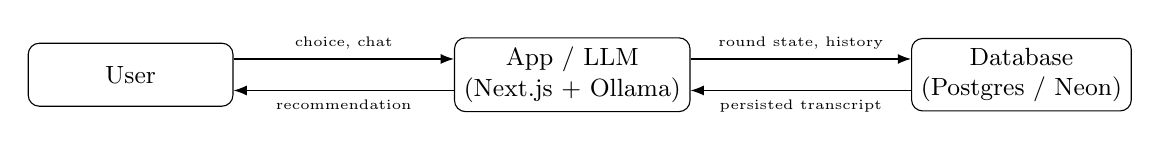
\begin{tikzpicture}[node distance=2.8cm, every node/.style={font=\small}, box/.style={draw, rounded corners, minimum width=2.6cm, minimum height=0.8cm, align=center}]
  \node[box] (user) {User};
  \node[box, right=of user] (app) {App / LLM\\(Next.js + Ollama)};
  \node[box, right=of app] (db) {Database\\(Postgres / Neon)};
  \draw[-{Latex}] ([yshift=2mm]user.east) -- node[above]{\tiny choice, chat} ([yshift=2mm]app.west);
  \draw[-{Latex}] ([yshift=-2mm]app.west) -- node[below]{\tiny recommendation} ([yshift=-2mm]user.east);
  \draw[-{Latex}] ([yshift=2mm]app.east) -- node[above]{\tiny round state, history} ([yshift=2mm]db.west);
  \draw[-{Latex}] ([yshift=-2mm]db.west) -- node[below]{\tiny persisted transcript} ([yshift=-2mm]app.east);
\end{tikzpicture}
\end{center}
The app assembles each round's context (traffic state, network topology, proposed routes, optimal distribution, user info, history buffer) from the database, sends it to the LLM component, and persists the resulting recommendation/transcript back to the database for the next round and for later metrics computation.

\section*{5. Action Items}
\begin{itemize}[label=$\square$]
  \item \textbf{Report on existing work}: document the current architecture (\texttt{lib/agent/recommend.ts}, \texttt{prompts.ts}, \texttt{ollama.ts}, \texttt{context.ts}), the framework in use (Next.js/TypeScript, Ollama for local LLM inference, Postgres/Neon for persistence), and the specific process by which this pipeline was turned into the PersuLLM-1 baseline.
  \item \textbf{Compute metrics} over the PersuLLM-1 experiments already run (gap-to-optimal, compliance, speed, judge-scored persuasiveness/logical coherence).
  \item \textbf{Start implementing RegConSuader} (Configurator, Strategy Selector, Persuader, Decider).
  \item \textbf{Begin the State-of-the-Art report}.
  \item \textbf{Draft the plan for the PFE report}.
\end{itemize}

\end{document}
